\section{Experiments}
\label{simulations}

\subsection{Overview}

We demonstrate the utility of these approaches using simulations. Each simulation is defined by a data-generating process with a known effect function, which allows us to compute true test set errors. Each run of each simulation generates a dataset, which we split into training and test samples. We perform $5$-fold cross validation on the training data and compute each model selection metric on each validation fold. I.e. for each training fold, we estimate $M$ different treatment effect functions $\hat\tau_m$ and for each of those we calculate each metric using the data in the corresponding validation fold. The metrics are averaged for each model across all folds. Each model selection approach then selects the model among the $M$ models that minimizes (or maximizes, when appropriate) its corresponding metric. The models selected by each approach on the basis of cross-validation are refit on the full training data and applied to the test set. The test-set treatment effect estimates of each model are compared to the known effects to calculate the true cost of using each approach for model selection. Each simulation is repeated multiple times. All of the code used to set up, run, and analyze the simulations is feely available on \href{https://github.com/som-shahlab/ITE-model-selection}{github}.

\subsubsection{Data-generating processes and sampling}

We use the sixteen simulations from \citet{Powers:2017wd}, each of which we repeat $100$ times. In each repetition, $1000$ samples are used for training ($\mathcal{T}$), $1000$ for validation ($\mathcal{V}$), and $1000$ for testing ($\mathcal{S}$). Let the data be denoted by $\{\bm y, \bm w, \bm x\} = \{[y_1 \dots y_n]^T, [w_1 \dots w_n]^T, [x_1 \dots x_n]^T\}$ where $n = |\mathcal{T}| + |\mathcal{V} | + |\mathcal{S}|$. Let $\bm y^{(\mathcal A)}$ represent $[y_i | i \in \mathcal A]$. Let the set of treated individuals be $\mathcal W_1 = \{i | w_i =1\}$ and let the set of untreated individuals be $\mathcal W_0 = \{i | w_i =0\}$.

\subsubsection{Models}

We fit several treatment effect models to each simulated dataset using the S-, T- and R-learning frameworks. Let $f(\bm x) = [f(x_i) \dots f(x_n)]$.

\paragraph{S-learners} We fit a variety of S-learners to each simulated dataset by regressing $\bm y^{(\mathcal T)}$ onto $[\bm x^{(\mathcal T)}, \bm z^{(\mathcal T)}]$ to produce $\hat\mu(x,w)$. The term $\bm z^{(\mathcal T)}$ is determined by $z_i = ( w_i- 0.5) x_i$ and ensures that the treatment effect is not implicitly regularized \cite{Nie:2017vi}. The treatment effect is calculated as $\hat\tau(x) = \hat\mu(x,1) - \hat\mu(x,0)$. 

The learning algorithms we use to fit $\hat\mu$ are gradient boosted trees (number of trees ranging from $1$ to $500$, tree depth of $3$, shrinkage of $0.2$ and minimum $3$ individuals per node) and elastic nets ($\alpha=0.5$, $\lambda \in [e^{-5}, e^2]$). These models give us a range of high-performing linear and nonlinear models to select among. We estimate a treatment effect model $\hat\tau_m(x)$ for each combination of algorithm and hyperparameters.

\paragraph{T-learners} T-learners are fit by separately regressing $\bm y^{(\mathcal T \cap \mathcal W_0)}$ onto $\bm x^{(\mathcal T \cap \mathcal W_0)}$ to estimate $\hat\mu_0(x)$ and $\bm y^{(\mathcal T \cap \mathcal W_0)}$ onto $\bm x^{(\mathcal T \cap \mathcal W_0)}$ to estimate $\hat\mu_1(x)$. The treatment effect is calculated as $\hat\tau(x) = \hat\mu_1(x) - \hat\mu_0(x)$. 

We use the same algorithms and hyperparameters as above to fit the models $\hat\mu_w(x)$. When estimating the various treatment effect models $\hat\tau_m(x)$, we only consider combinations of models $\hat\mu_1$ and $\hat\mu_0$ that were fit using the same algorithm with the same hyperparameters. This increases computational efficiency, but need not be done in practice (i.e. $\hat\mu_0$ could be fit using a linear model and $\hat\mu_1$ fit using a random forest). It is an appropriate simplification to make in our experiments since our focus is on model selection and not model fitting.

\paragraph{R-learners} In the R-learning framework of \citet{Nie:2017vi}, treatment effect models are estimated by minimizing 

\begin{equation}
	\frac{1}{|\mathcal{T}|}\sum_{i \in \mathcal{T}}^{|\mathcal{T}|}  
	((y_i - \hat m(x_i)) - (w_i - \hat p(x_i))t(x_i))^2
\label{r-learner}
\end{equation}

over a space of candidate models $t(x)$. Given $\hat m(x)$ and $\hat p(x)$, this is equivalent to a weighted least-squares problem with a pseudo-outcome of $\frac{ y_i - \hat m(x_i) }{w_i - \hat p(x_i)}$ and weights of $(w_i - \hat p(x_i))^2$. As such, it can be solved using a variety of learning algorithms. 

In our experiments, we estimate the quantities $\hat m(\bm x^{(\mathcal T)})$ and $\hat p(\bm x^{(\mathcal T)})$ using cross-validated cross-estimation over the training set \cite{Nie:2017vi, Wager:2016dz}. The internal cross-validation is run over estimates derived from the same combinations of algorithms and hyperpameters as used by the S- and T-learners. These estimates are then fixed and used for all R-learners. Each R-learner $\hat\tau_m(x)$ is then produced by minimizing equation \ref{r-learner} using a different learning algorithm and set of hyperparameters. We use the same combinations of algorithms and hyperpameters as used by the S- and T-learners.

\subsubsection{Model selection metrics}

The following metrics are used to select among models in each simulation:

% This table is terrible. Need to 1) get Type to be multicolumn 2) fix vertical spacing b/t lines 3) make Ref section much thinner

\begin{center}
\tabulinesep=1mm
\begin{tabu}{|l|c|}
	\hline
	 \rowfont[c]{\bfseries} Metric & Reference  \\
	 \hline
	 Random 						& NA  \\
	 $\widehat{\mu\text{-risk}}$		& \ref{murisk}  \\
	 $\widehat{\mu\text{-risk}}_{IPTW}$	& \ref{murisk-iptw} \\
	 $\hat v_{IPTW}$ 				& \ref{value}  \\
	 $\hat v_{DR}$					& \ref{value-dr} \\
	 $\widehat{\tau\text{-risk}}_{match}$	& \ref{trisk-match} \\
	 $\widehat{\tau\text{-risk}}_{IPTW}$ 	& \ref{trisk-iptw} \\
	 $\widehat{\tau\text{-risk}}_{R}$		& \ref{trisk-r} \\
	 \hline
\end{tabu}
\end{center}

Taking the model that minimizes (or maximizes, when appropriate) one of these metrics defines a model selection approach. 

The ``random'' approach selects a model uniformly at random from the available models. 

Several of these metrics require estimates $\check p(\bm x^{(\mathcal V)})$, $\check \mu_w(\bm x^{(\mathcal V)})$, or $\check m(\bm x^{(\mathcal V)})$. In our experiments, we estimate each of these quantities using cross-validated cross-estimation over the validation set alone. The internal cross-validation is run over estimates derived from the same combinations of algorithms and hyperpameters as used by the treatment effect learners. 

\subsubsection{Evaluation metrics}

Let the model $\hat\tau_m$ selected by optimizing metric $h$ be written as $\hat\tau^{*_h}$. 

We are interested in the quantities

\[
\tau\text{-risk}_h = E[ (\hat\tau^{*_h} (X) - \tau(X))^2 ]
\]

and 

\[
v_h = E[ Y| W =\hat d^{*_h} (X)]
\]

which we unbiasedly estimate in a large test set $\mathcal{S}$ via

\begin{equation}
\label{true-mse}
\tau\text{-risk}^{(\mathcal{S})}_h = \frac{1}{|\mathcal{S}|}\sum_{i \in \mathcal{S}} (\hat\tau^{*_h} (x_i) - \tau(x_i))^2
\end{equation}

and 

\begin{equation}
\label{true-value}
v^{(\mathcal{S})}_h = \frac{1}{|\mathcal{S}|}\sum_{i \in \mathcal{S}} \mu_{\hat d^{*_h}(x_i)}(x_i)
\end{equation}

Where $\hat d^{*_h}(x_i) = I(\hat\tau^{*_h}(x_i) > 0)$ as before. 

$\tau\text{-risk}_{h}^{(\mathcal{S})}$ calculates how well the selected model estimates the treatment effect for individuals in the test set. $v^{(\mathcal{S})}$ is the decision value of applying the treatment policy $\hat d(x)$ derived from each selected model to the individuals in the test set.

These are both useful metrics, although only the first ($\tau\text{-risk}$), sometimes called ``precision in estimating heteorgenous effects'', or PEHE) has typically been used in simulation studies in the individual effect estimation literature while $v^{(\mathcal{S})}$ is used in the policy learning literature. To see why they are both important, consider two models ($A$ and $B$) that estimate the same treatment effect for all individuals, except for two individuals ($i=1$ and $i=2$). Let $\tau(x_1) = \tau(x_2) = 0.1$, i.e. both individuals would benefit from the treatment in reality. Model $A$ estimates $\hat\tau_A(x_1) = -0.1$ and $\hat\tau_A(x_2) = 0.1$. In other words, it incorrectly suggests not treating individual $1$, although the absolute difference $|\hat\tau_A(x_1)-\tau(x_1)| = 0.2$ is quite small, so it is not heavily penalized according to $\tau\text{-risk}$. Model $B$ estimates $\hat\tau_B(x_1) = 0.1$ and $\hat\tau_B(x_2) = 100$. Model $B$ correctly suggests the treatment for both individuals, but the absolute difference $|\hat\tau_B(x_2)-\tau(x_2)| = 99.9$ is large and is heavily penalized by $\tau\text{-risk}$. Often, what we want is a model that correctly assigns treatment to the individuals who stand to benefit from it. Using $\tau\text{-risk}$ in this case would favor model $A$ even though it leads to the mistreatment of more individuals than model $B$ does. However, $\tau\text{-risk}$ is still a useful metric. There may be cases where a researcher is interested in the precise magnitude of the effect for each individual, perhaps so that scarce resources can be allocated most effectively. 

\begin{comment}

In our simulations, we also calculate the optima of both $v^{(\mathcal{S})}$ and $\tau\text{-risk}^{(\mathcal{S})}$ over all the computed models $\hat\tau_m \in \{\hat\tau_1 \dots \hat\tau_M\}$:

\[
\tau MSE^{(\mathcal{T})}_{*} = \underset{m}{\text{min}} \ \ \frac{1}{|\mathcal{T}|}\sum_{i \in \mathcal{T}} (\hat\tau_m (x_i) - \tau(x_i))^2
\]

\[
v^{(\mathcal{T})}_{*} = \underset{m}{\text{max}} \ \ \frac{1}{|\mathcal{T}|}\sum_{i \in \mathcal{T}} \mu_{\hat d_m(x_i)}(x_i)
\]

These quantities represent the best possible performance that any model selection method could achieve given the available models in a given simulation. We use these quantities as baselines.

We also calculate these using the true model $\hat\tau = \tau$, which represents the best achievable performance without specifying any models a-priori:

\[
\tau MSE^{(\mathcal{T})}_{**} = 0
\]

\[
v^{(\mathcal{T})}_{**} = \frac{1}{|\mathcal{T}|}\sum_{i \in \mathcal{T}} \mu_{ d(x_i)}(x_i)
\]

We use these minima to calculate the improvements obtained by each model selection approach relative to optimal baselines, which allows for comparison between different simulations. The relative values of $\tau MSE^{(\mathcal{T})}_{h}$ and $C^{(\mathcal{T})}_{h}$ within one test set and one set of models are

\[
	R\text{-} \tau MSE^{(\mathcal{T})}_{h} = 
	\frac{\tau MSE^{(\mathcal{T})}_{h} - \tau MSE^{(\mathcal{T})}_{**}}{\tau MSE^{(\mathcal{T})}_{*} - \tau MSE^{(\mathcal{T})}_{**}}
\]

\[
	R\text{-}  v^{(\mathcal{T})}_{h} = 
	\frac{ v^{(\mathcal{T})}_{h} -  v^{(\mathcal{T})}_{**}}{ v^{(\mathcal{T})}_{*} -  v^{(\mathcal{T})}_{**}}
\]

The closer to zero these are, the better the performance of the model selection method.
\end{comment}

\subsection{Results}

% latex table generated in R 3.2.2 by xtable 1.7-4 package
% Wed May  9 15:03:55 2018
\begin{table}[ht]
\centering
\caption{$\tau\text{-risk}^{(\mathcal{S})}$. True test-set $\tau\text{-risk}$ of the treatment effect model selected according to each metric (rows) in each simulation (columns), averaged across replications. Simulations 9-16 use the same data-generating functions as 1-8, but with nonrandom treatment assignment. Smaller numbers indicate better performance.}
\begin{tabular}{lllllllll}
  \hline
metric & 1 & 2 & 3 & 4 & 5 & 6 & 7 & 8 \\ 
  \hline
Random & 0.102 & 2.684 & 2.223 & 1.718 & 1.233 & 2.845 & 5.859 & 2.677 \\ 
  $\widehat{\mu\text{-risk}}$ & \bfseries{0.007} & 0.235 & \bfseries{0.014} & 0.808 & 0.212 & 0.963 & 2.970 & 1.738 \\ 
  $\widehat{\mu\text{-risk}}_{IPTW}$ & \bfseries{0.007} & 0.235 & \bfseries{0.014} & 0.808 & 0.212 & 0.963 & 2.970 & 1.738 \\ 
  $\hat v_{IPTW}$ & 0.130 & 0.634 & 4.278 & 0.690 & 0.738 & 0.887 & 4.300 & 1.513 \\ 
  $\hat v_{DR}$ & 0.052 & 0.969 & 8.458 & 0.785 & 4.466 & 0.972 & 5.759 & 2.577 \\ 
  $\widehat{\tau\text{-risk}}_{match}$ & 0.013 & 0.542 & 0.964 & 0.068 & 0.260 & 0.970 & 3.681 & 0.815 \\ 
  $\widehat{\tau\text{-risk}}_{IPTW}$ & 0.056 & 0.101 & 0.050 & 0.154 & 0.288 & \bfseries{0.786} & 2.913 & 0.746 \\ 
  $\widehat{\tau\text{-risk}}_{R}$ & 0.008 & \bfseries{0.059} & 0.017 & \bfseries{0.035} & \bfseries{0.043} & \bfseries{0.786} & \bfseries{2.794} & \bfseries{0.736} \\ 
  \hline
   \\
  \\
  \hline
metric & 9 & 10 & 11 & 12 & 13 & 14 & 15 & 16 \\ 
  \hline
Random & 0.401 & 3.178 & 61.830 & 4.143 & 4.173 & 3.019 & 8.899 & 4.235 \\ 
  $\widehat{\mu\text{-risk}}$ & 0.012 & 0.290 & \bfseries{0.020} & 0.797 & \bfseries{0.055} & 1.277 & \bfseries{3.900} & 2.495 \\ 
  $\widehat{\mu\text{-risk}}_{IPTW}$ & 0.013 & \bfseries{0.288} & 0.040 & 0.782 & 0.060 & 1.250 & 4.050 & 2.277 \\ 
  $\hat v_{IPTW}$ & 0.822 & 1.290 & 4.542 & 1.677 & 5.247 & 1.274 & 6.174 & 2.431 \\ 
  $\hat v_{DR}$ & 0.146 & 1.169 & 5.678 & 1.821 & 26.571 & 1.356 & 7.340 & 2.668 \\ 
  $\widehat{\tau\text{-risk}}_{match}$ & 0.400 & 1.617 & 4.400 & 1.769 & 9.399 & 1.425 & 4.284 & 1.661 \\ 
  $\widehat{\tau\text{-risk}}_{IPTW}$ & 1.049 & 0.451 & 2.387 & 1.129 & 4.260 & \bfseries{1.120} & 4.133 & 2.123 \\ 
  $\widehat{\tau\text{-risk}}_{R}$ & \bfseries{0.008} & 0.348 & 1.986 & \bfseries{0.149} & 0.078 & 1.169 & 3.923 & \bfseries{1.539} \\ 
     \hline
\end{tabular}
\label{tmse-table}
\end{table}

% latex table generated in R 3.2.2 by xtable 1.7-4 package
% Wed May  9 15:04:17 2018
\begin{table}[ht]
\centering
\caption{$v^{(\mathcal{S})}$. True test-set value of the decision rule derived from the treatment effect model selected according to each metric (rows) in each simulation (columns), averaged across replications. Simulations 9-16 use the same data-generating functions as 1-8, but with nonrandom treatment assignment. Larger numbers indicate better performance.}
\begin{tabular}{lllllllll}
  \hline
metric & 1 & 2 & 3 & 4 & 5 & 6 & 7 & 8 \\ 
  \hline
Random & \bfseries{0.008} & 0.501 & 1.914 & 0.791 & 0.771 & 0.446 & 0.138 & 0.685 \\ 
  $\widehat{\mu\text{-risk}}$ & \bfseries{0.008} & 0.795 & \bfseries{1.998} & 0.966 & 0.906 & 0.663 & 0.642 & 0.835 \\ 
  $\widehat{\mu\text{-risk}}_{IPTW}$ & \bfseries{0.008} & 0.795 & \bfseries{1.998} & 0.966 & 0.906 & 0.663 & 0.642 & 0.835 \\ 
  $\hat v_{IPTW}$ & \bfseries{0.008} & 0.798 & 1.989 & 0.969 & 0.877 & \bfseries{0.678} & 0.651 & 0.842 \\ 
  $\hat v_{DR}$ & \bfseries{0.008} & 0.770 & 1.978 & 0.969 & 0.486 & 0.667 & 0.354 & 0.784 \\ 
  $\widehat{\tau\text{-risk}}_{match}$ & \bfseries{0.008} & 0.783 & 1.998 & 0.984 & 0.903 & 0.671 & 0.505 & 0.881 \\ 
  $\widehat{\tau\text{-risk}}_{IPTW}$ & \bfseries{0.008} & 0.806 & 1.997 & 0.979 & 0.890 & 0.678 & 0.672 & \bfseries{0.884} \\ 
  $\widehat{\tau\text{-risk}}_{R}$ & \bfseries{0.008} & \bfseries{0.809} & 1.998 & \bfseries{0.986} & \bfseries{0.907} & 0.678 & \bfseries{0.687} & 0.883 \\ 
  \hline
   \\
  \\
  \hline
metric & 9 & 10 & 11 & 12 & 13 & 14 & 15 & 16 \\ 
  \hline
Random & \bfseries{-0.011} & 0.407 & 1.852 & 0.505 & 0.680 & 0.421 & 0.157 & 0.586 \\ 
  $\widehat{\mu\text{-risk}}$ & \bfseries{-0.011} & 0.762 & \bfseries{1.993} & 0.945 & \bfseries{0.906} & 0.653 & 0.532 & 0.709 \\ 
  $\widehat{\mu\text{-risk}}_{IPTW}$ & \bfseries{-0.011} & 0.761 & 1.993 & 0.945 & 0.906 & 0.653 & 0.505 & 0.725 \\ 
  $\hat v_{IPTW}$ & \bfseries{-0.011} & 0.721 & 1.923 & 0.881 & 0.562 & \bfseries{0.656} & \bfseries{0.593} & 0.751 \\ 
  $\hat v_{DR}$ & \bfseries{-0.011} & 0.703 & 1.969 & 0.945 & 0.142 & 0.654 & 0.177 & 0.671 \\ 
  $\widehat{\tau\text{-risk}}_{match}$ & \bfseries{-0.011} & 0.494 & 1.960 & 0.861 & 0.126 & 0.647 & 0.481 & 0.790 \\ 
  $\widehat{\tau\text{-risk}}_{IPTW}$ & \bfseries{-0.011} & 0.740 & 1.966 & 0.921 & 0.598 & 0.653 & 0.579 & 0.786 \\ 
  $\widehat{\tau\text{-risk}}_{R}$ & \bfseries{-0.011} & \bfseries{0.777} & 1.983 & \bfseries{0.995} & 0.904 & 0.655 & 0.547 & \bfseries{0.806} \\ 
   \hline
\end{tabular}
\label{value-table}
\end{table}

\begin{figure}
  \centering
    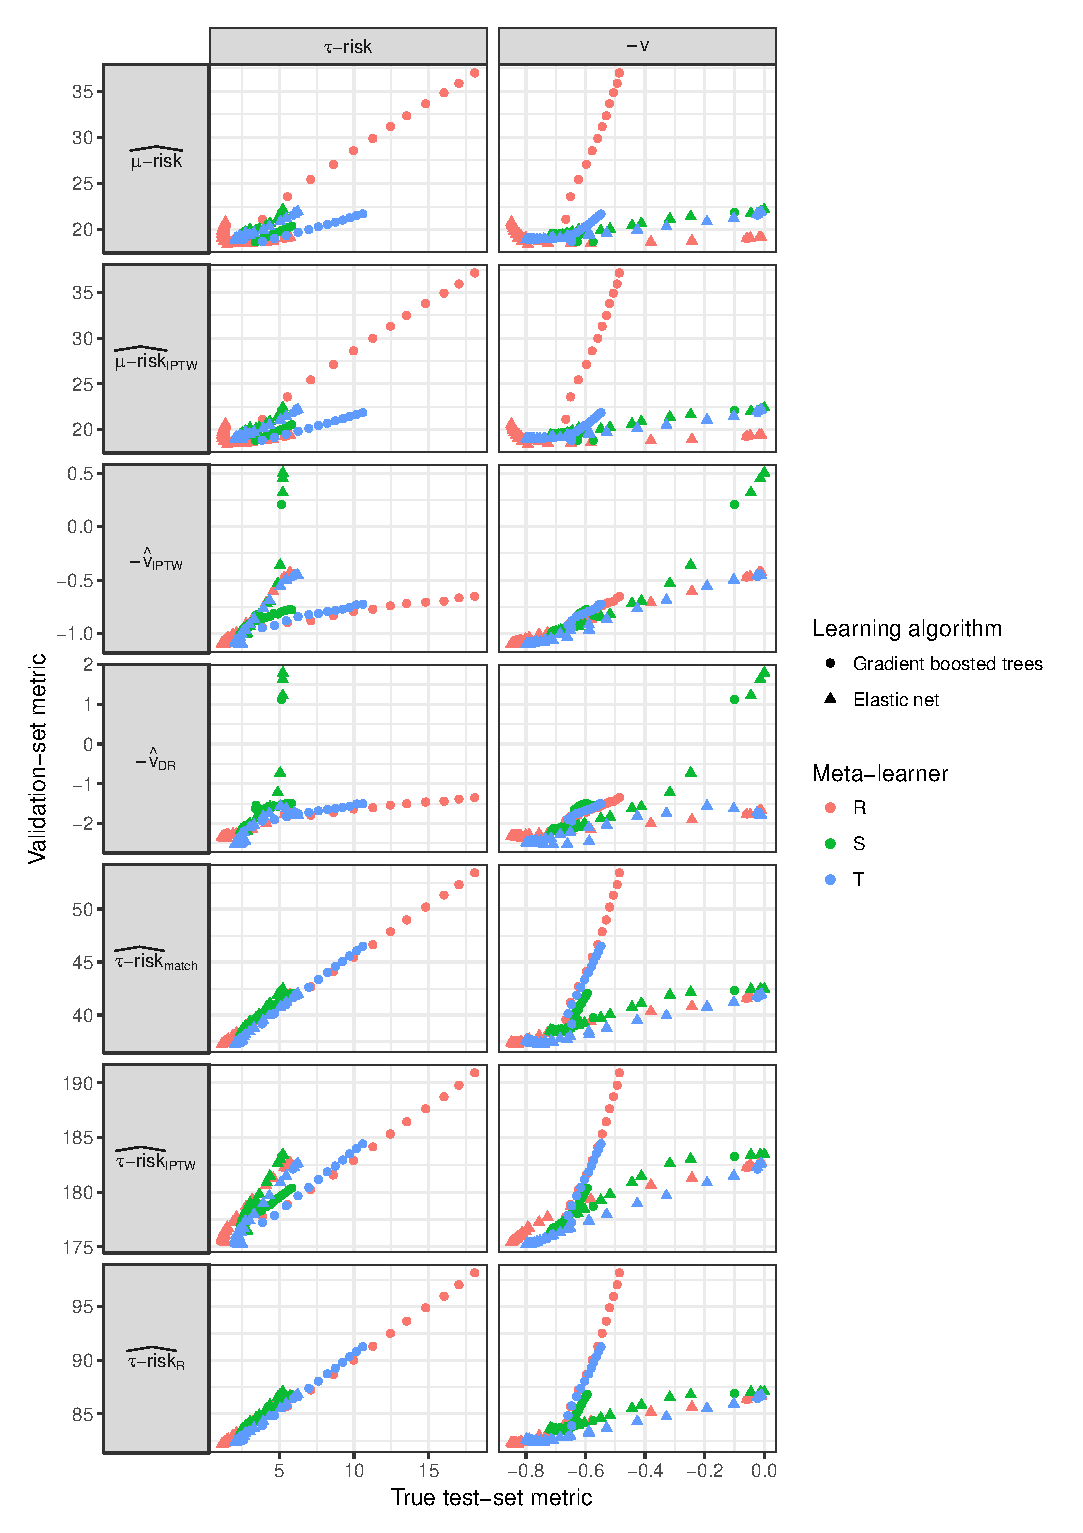
\includegraphics[width=\textwidth]{detailed_results_sim16}
      \caption{Validation-set and test-set metrics for all treatment effect models, averaged over all replications of simulation 16 (equivalent plots for other simulations show the same patterns). Each point is a single model resulting from a unique combination of meta-learner (S, T, or R), learning algorithm, and hyperparameters. The x-axis facets are the values of $\tau\text{-risk}^{(\mathcal{S})}$ and $-v^{(\mathcal{S})}$ for each model (lower values indicating higher performance). The y-axis facets are the model selection metrics for each model as estimated on the validation set (lower values indicating higher predicted performance). High correlation between a validation-set and test-set metric indicates good performance of the model selection metric.}
      \label{details16}
\end{figure}

The results in tables \ref{tmse-table} and \ref{value-table} show that $\widehat{\tau\text{-risk}}_{R}$ is the metric that most consistently selects models with low $\tau\text{-risk}$ and high value. This is especially true when treatment assignment is randomized, but also to a large extent when the assignment is biased. In the simulations where other model selection approaches win out, it is typically by a small margin. Both $\widehat{\mu\text{-risk}}$ and $\widehat{\mu\text{-risk}}_{IPTW}$ perform well (the two are identical in randomized settings). Even when the goal is to optimize value, selecting on the basis of these metrics leads to better performance than using $\hat v_{IPTW}$ or $\hat v_{DR}$. Figure \ref{details16} shows the results from simulation 16 in greater detail.


